%%==============================================================================
%% 第 2 章 人机协作动态任务规划建模
%%==============================================================================
\chapter{人机协作动态任务规划建模}\label{chap:method}

\section{引言}
本章将人机协作任务规划问题形式化为马尔可夫决策过程，并给出状态、动作与奖励的
定义。

\section{马尔可夫决策过程建模}
将人机协作系统建模为五元组 $\mathcal{M}=(\mathcal{S},\mathcal{A},P,R,\gamma)$，
其中 $\mathcal{S}$ 为状态空间，$\mathcal{A}$ 为动作空间，$P$ 为状态转移概率，
$R$ 为奖励函数，$\gamma\in(0,1]$ 为折扣因子。智能体的目标是最大化累积折扣
回报，如式~\eqref{eq:return} 所示：
\begin{equation}\label{eq:return}
  G_t = \sum_{k=0}^{\infty} \gamma^{k} R_{t+k+1}.
\end{equation}

最优策略 $\pi^{*}$ 满足贝尔曼最优方程~\eqref{eq:bellman}：
\begin{equation}\label{eq:bellman}
  Q^{*}(s,a) = \mathbb{E}\!\left[ R_{t+1}
    + \gamma \max_{a'} Q^{*}(s',a') \,\middle|\, s,a \right].
\end{equation}

\begin{definition}[协作安全裕度]\label{def:safety}
设人与机器人末端的最小距离为 $d_{\min}$，安全阈值为 $d_{s}$，则协作安全裕度
定义为 $\eta = (d_{\min}-d_{s})/d_{s}$。
\end{definition}

\begin{theorem}\label{thm:converge}
在折扣因子 $\gamma<1$ 且奖励有界的条件下，值迭代算法收敛到唯一最优值函数。
\end{theorem}
\begin{proof}
由 Bellman 最优算子的 $\gamma$-压缩性质，结合 Banach 不动点定理即可证得，
此处从略。
\end{proof}

\section{系统框架}
本文提出的动态任务规划系统框架如图~\ref{fig:framework} 所示。系统由感知模块、
决策模块与执行模块组成。

\begin{figure}[htbp]
  \centering
  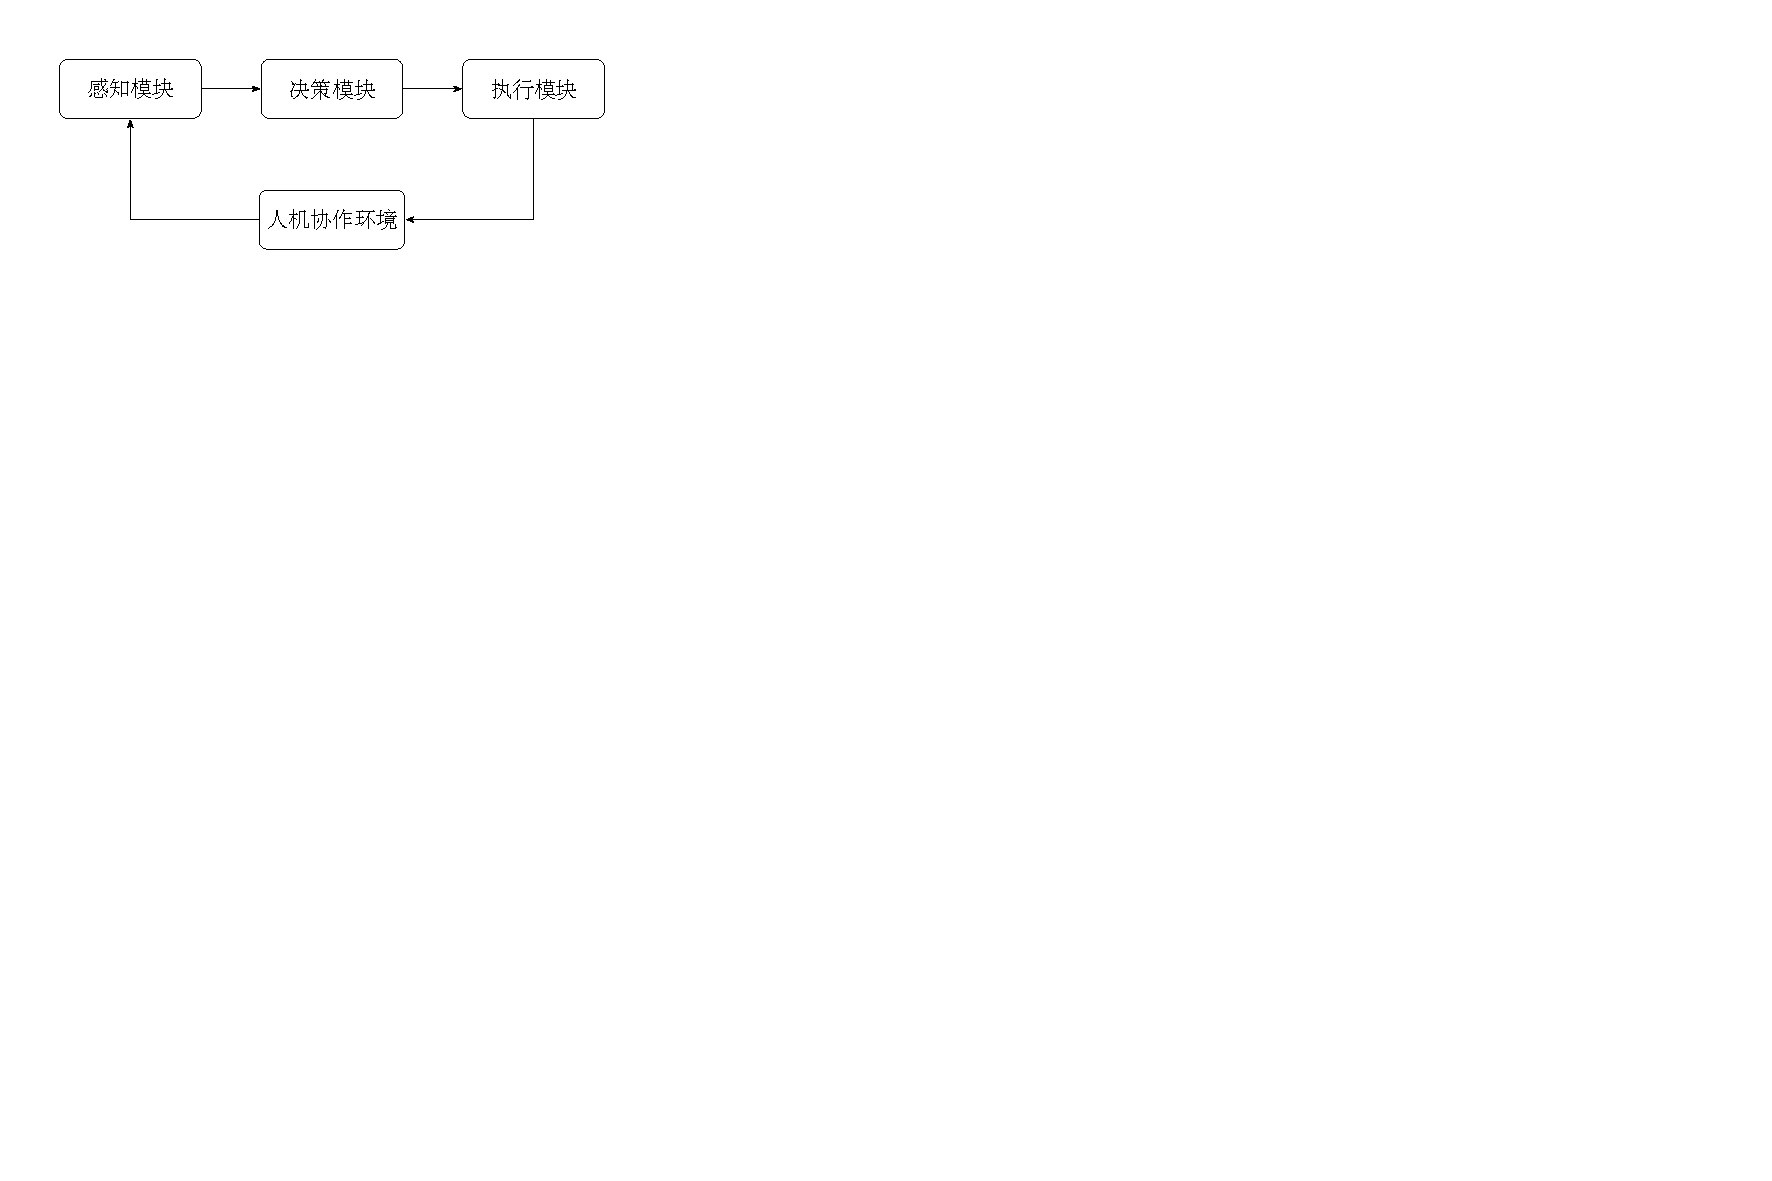
\includegraphics[width=0.7\textwidth]{figures/example-figure.pdf}
  \caption{人机协作动态任务规划系统框架}
  \label{fig:framework}
\end{figure}

\section{本章小结}
本章建立了人机协作动态任务规划的马尔可夫决策过程模型，给出了协作安全裕度的
定义，并证明了值迭代算法的收敛性，为后续算法设计奠定了基础。
